\documentclass[onecolumn, 12pt]{book}

\usepackage[latin1]{inputenc}   
\usepackage{amsmath}
\usepackage{algorithm}
\usepackage{algorithmic} 
%\usepackage[T1]{fontenc}

%\usepackage[francais]{babel}     
\usepackage{layout}    
\usepackage[top=2cm, bottom=2cm, left=2cm, right=2cm]{geometry} 
\usepackage{setspace}
\usepackage{soul}
\usepackage{color} 
\usepackage{verbatim}
\usepackage{moreverb}
\usepackage{listings}
\usepackage{url}
\usepackage{graphicx}
%\usepackage{epstopdf}
%\usepackage[outdir=/home/willy/Documents/latexDoc/redactionThese/fusion_fichiers/images_fusionChapitres/]{epstopdf}
%\usepackage[outdir=./../../fusion_fichiers/images_fusionChapitres/]{epstopdf}
\usepackage[outdir=./]{epstopdf}
\usepackage{caption}
\usepackage{setspace}
 
 
% \title{Mod\`ele de Donn\'ees}
% \author{Willy Ehounou}
 %\date{01/06/15}
\title{Chapitre6 : Simulations sur donn\'ees al\'eatoires}
\author{Wilfried Ehounou}
\date{\oldstylenums{\today}} 

\newtheorem{definition}{D\'efinition}
\newtheorem{theorem}{Theorem}
\newtheorem{property}{Propri\'et\'e}
\newtheorem{claim}[theorem]{Claim}
\newtheorem{proposition}[theorem]{Proposition}
\newtheorem{lemma}[theorem]{Lemma}
\newtheorem{corollary}[theorem]{Corollary}
\newtheorem{conjecture}[theorem]{Conjecture}
\newtheorem{observation}{Observation}
\newtheorem{example}{Exemple}
\newtheorem{remark}{Remark}

%---- path figures ----
\graphicspath{{/home/willy/Documents/courbePython/courbeDegreCoutMinAleatoire_11_09_2017/}
{/home/willy/Documents/courbePython/courbeDegreCoutMinAleatoire_11_10_2017/}
{/home/willy/Documents/courbePython/courbeDegreCoutMinAleatoire_11_09_2017/comparaison_MethodesCorrection_fctDeCout_permut_aleatoire_coutMin_degreMin/}
{/home/willy/Documents/latexDoc/redactionThese/fusion_fichiers/images_fusionChapitres/}
}
 
\begin{document}
\maketitle
\tableofcontents

\chapter{Simulation des algorithmes sur des r\'eseaux th\'eoriques}
Dans ce chapitre, nous allons proc\'eder de mani\`ere contraire au probl\`eme \`a resoudre en supposant que les r\'eseaux \'electriques de flots sont connus. 
%Les algorithmes precedents sont test\'es sur des r\'eseaux de flots g\'en\'er\'es qui simulent le fonctionnement d'un r\'eseau \'electrique de Datacenter.
\`A partir de ces r\'eseaux, nous produisons leurs line graphes associ\'es et en d\'eduisons leurs matrices d'adjacences. 
Nous modifions certains valeurs dans ces matrices pour introduire des erreurs d'adjacences entre ar\^etes. \newline
Nous attribuons les corr\'elations entre ar\^etes \`a partir de diff\'erentes lois de distributions, tout en tenant compte des erreurs de corr\'elations introduites dans ces matrices d'adjacences. \newline
Les algorithmes propos\'es sont ex\'ecut\'es sur des matrices de corr\'elation construites par les corr\'elations entre ar\^etes et nous allons comparer les line graphes produites par les algorithmes avec ceux d\'eduits des r\'eseaux \'electriques de flots. 


\section{Objectifs}
Les travaux r\'ealis\'es dans cette partie ont pour but de montrer que les algorithmes propos\'es (couverture et correction) fournissent un line graphe de distance de Hamming minimale lorsque la matrice d'adjacence de ce graphe contient plus de corr\'elations {\em fausses positives} que de corr\'elations {\em fausses n\'egatives} et peu d'erreurs de corr\'elations et cela malgr\'e l'ordre du line graphe. Pr\'ecisons aussi le nombre d'erreurs de corr\'elation  doit \^etre inf\'erieur \`a $6$ pour un seuil de corr\'elation sup\'erieure \`a $0.8$ . \newline
Pour parvenir \`a un tel resultat, nous montrons que les sommets, n'appartenant \`a aucune couverture (sommets $\in sommets\_1$) doivent \^etre corrig\'es avec la m\'ethode de {\bf permutation al\'eatoire minimum} pour une {\bf fonction de co\^ut normale} pour de meilleurs r\'esultats.
Nous montrons \'egalement la relation existante entre la distance de Hamming et la distance line.

\section{D\'efinitions}
Soient le graphe non orient\'e $G$ du r\'eseau de flots, le line graphe $LG$ associ\'e \`a $G$ et la matrice d'adjacence $matE$ de $LG$. La matrice de corr\'elation entres ar\^etes de $G$, appliqu\'ee \`a une valeur de seuil, donne la matrice d'adjacence $matE$ dont les sommets sont les ar\^etes de $G$. \newline
Le line graphe dont on ajoute des erreurs de corr\'elations (modification de cases) dans sa matrice d'adjacence est not\'e $LG'$. La matrice d'adjacence de $LG'$ est $matE'$. 

\begin{definition}
Une corr\'elation entre ar\^etes (ou arcs) est l'existence d'un sommet commun aux ar\^etes (ou arcs). 
Ce sommet commun peut \^etre source, destination ou interm\'ediaire comme pr\'esent\'e dans la figure \ref{typeSommetEnCommun}
\begin{centering} 
\begin{figure}[htb!] 
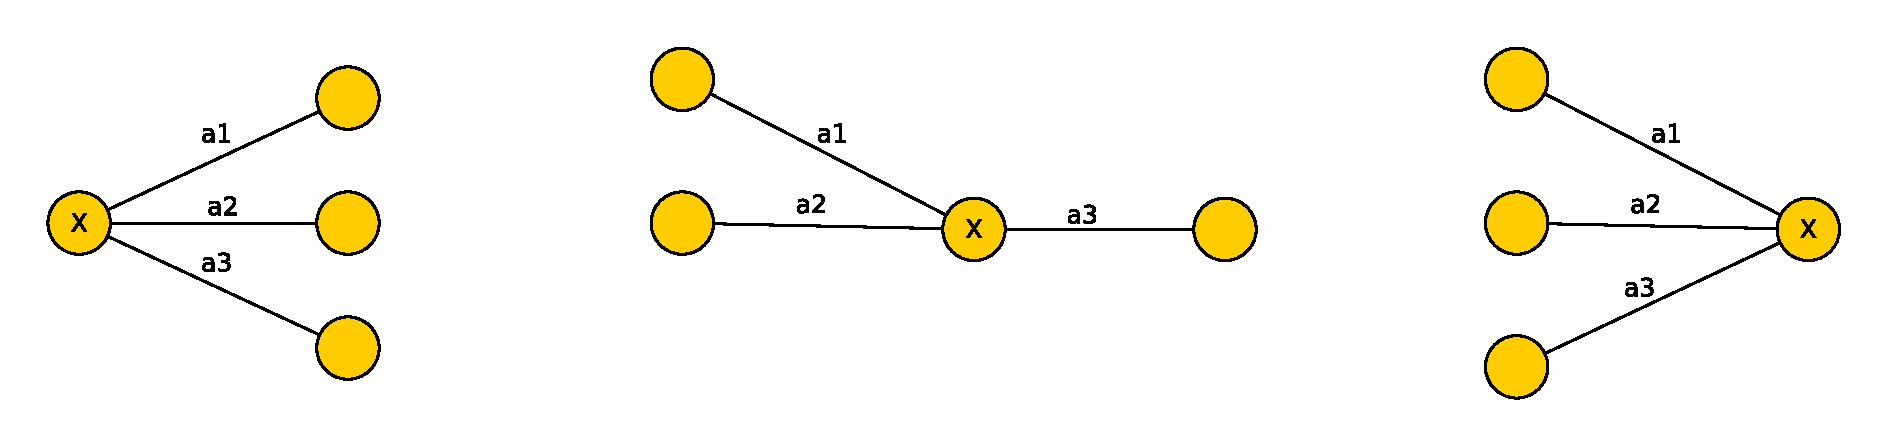
\includegraphics[scale=0.50]{typeSommetsEnCommun.eps}
\caption{De la gauche \`a la droite: sommet $X$ source, sommet $X$ interm\'ediaire, sommet $X$ destination}
\label{typeSommetEnCommun} 
\end{figure}
\end{centering} 
\end{definition}
Dans la matrice d'adjacence $matE$ du line graphe form\'e par les corr\'elations, chaque case re\c coit $1$ quand deux ar\^etes partagent un sommet alors que la case re\c coit $0$ dans le cas contraire.

\begin{definition}
%Une {\bf erreur de corr\'elation} est l'existence de corr\'elation entre deux ar\^etes (arcs) lorsqu'il n'existe pas de corr\'elation ou l'absence de corr\'elation lorsque il en existe une.
Une {\bf erreur de corr\'elation} est la modification de la valeur d'une case de la matrice d'adjacence $matE$ de $LG$.
\end{definition}
On distingue quatre cat\'egories d'erreurs de corr\'elation, regroup\'ees dans le tableau \ref{categoriesErreursCorrelation}. Il s'agit des corr\'elations 
\begin{itemize}
\item {\bf vrai positives} : Il s'agit de cases \`a $1$ n'ayant pas \'et\'e modifi\'ees dans la matrice $matE$.
\item {\bf vrai n\'egatives} :  Il s'agit de cases \`a $0$ n'ayant pas \'et\'e modifi\'ees dans la matrice $matE$.
\item {\bf faux positives} : Il s'agit de cases \`a $0$ modifi\'ees dans la matrice $matE$.
\item {\bf faux n\'egatives} : Il s'agit de cases \`a $1$ modifi\'ees dans la matrice $matE$.
\end{itemize}

\begin{property}
 La corr\'elation {\em fausse n\'egative} (l'absence de corr\'elation) est d\'esign\'ee par la valeur $0$ dans la matrice d'adjacence $matE'$ tandis que la corr\'elation {\em fausse positive} (l'existence de corr\'elation) a une valeur $1$ dans cette matrice. (voir tableau \ref{categoriesErreursCorrelation})
\end{property}

\begin{table}[h]
	\centering
	\begin{tabular}{ p{3em} p{3em} p{10em} }
		$LG$ & $LG'$ & $\hspace{1 em}$ corr\'elations \\
		0 & 0 & $\rightarrow$ vrai n\'egative \\
		0 & 1 & $\rightarrow$ fausse positive \\
		1 & 0 & $\rightarrow$ fausse n\'egative \\
		1 & 1 & $\rightarrow$ vrai positive \\
	\end{tabular}
	\caption{ \label{categoriesErreursCorrelation} Valeurs de corr\'elations selon le type d'erreurs dans les matrices d'adjacence de $LG$ et $LG'$}
\end{table}

\begin{definition} {matrice de corr\'elation} \newline
% comment on obtient la matrice 
% de la matrice d'adjacence, on definit des lois de distribution pour chaque categorie d'erreurs de correlation
La matrice de corr\'elation est une matrice de relation entre ar\^etes dans laquelle, \`a chaque case, est associ\'e une valeur de probabilit\'e correspondante \`a la corr\'elation entre ces ar\^etes. 
\end{definition}
Les valeurs de probabilit\'es sont d\'efinies, en fonction du type d'erreurs de corr\'elation, par diff\'erentes lois de distributions. 
\newline
%%Nous consid\'erons {\bf l'hypoth\`ese de corr\'elations des arcs} suivante :
%{\em les corr\'elations entre arcs ou ar\^etes proche de $1$ ont plus de chance de partager  un sommet tandis que celles proche de $0$ ne partageront jamais de sommets}.
\begin{definition} : Hypoth\`ese de corr\'elations des arcs \newline
\label{hypotheseCorrelationArcs}
Les corr\'elations entre arcs ou ar\^etes, proche de $1$, ont tendance \`a partager  un sommet tandis que celles proche de $0$ ne partageront jamais de sommets
\end{definition}
\`A partir de la d\'efinition \ref{hypotheseCorrelationArcs}, nous d\'efinissons une valeur de seuil pour dissocier les ar\^etes adjacentes des ar\^etes non adjacentes. En effet les corr\'elations entre ar\^etes, inf\'erieure au seuil, sont transform\'ees en $0$ et celles, sup\'erieure ou \'egale au seuil, sont modifi\'ees par $1$ dans la matrice de corr\'elation. En appliquant la valeur de seuil, on transforme notre matrice probabiliste en une {\bf matrice de corr\'elation binaire} qui est aussi la matrice d'adjacence $matE$ entre ar\^etes du graphe $LG$. 

\begin{definition}{ m\'etrique: distance de Hamming} \newline
La m\'etrique utilis\'ee pour diff\'erencier deux graphes est la {\em distance de Hamming}.
La distance de Hamming est le nombre d'ar\^etes (ou arcs) diff\'erentes entre deux graphes ayant le m\^eme ensemble de sommets. 
\end{definition}
Ainsi, une distance de Hamming \'egale \`a $0$ signifie que les deux graphes sont identiques. Tandis que  une distance de Hamming \'egale \`a $k$ signifie qu'il a $k$ ar\^etes diff\'erentes entre ces deux graphes.

\begin{definition}{ fonction de co\^ut d'un sommet} \newline
La fonction de co\^ut d'un sommet est le co\^ut de chaque ar\^ete ajout\'ee ou supprim\'ee lorsqu'on applique l'algorithme de correction sur ce sommet.
\end{definition}
Le co\^ut d'une ar\^ete peut \^etre
\begin{itemize}
	\item unitaire : l'ajout et la suppression valent $1$.
	\item normal : la suppression co\^ute la corr\'elation entre l'ar\^ete et une autre et l'ajout vaut  $1$ moins cette corr\'elation.
	\item quadratique : la suppression co\^ute la corr\'elation au carr\'e entre l'ar\^ete et une autre  et l'ajout vaut  $1$ moins cette corr\'elation au carr\'e.
	\item puissance $4$ :  la suppression est la corr\'elation entre l'ar\^ete et une autre \`a la puissance $4$ et l'ajout vaut  $1$ moins cette corr\'elation \`a la puissance $4$.
	\item en cloche : l'ajout et la suppression dependent d'une fonction polynomiale de degr\'e $2$ dont les valeurs autour d'un seuil sont proche de $0$. Nous y reviendrons dans la partie \ref{fonctionDeCout} 
\end{itemize}

\section{Donn\'ees: G\'en\'eration al\'eatoires de graphes} 

\subsection{G\'en\'eration de r\'eseaux de flots}
La structure de donn\'ees utilis\'ee, pour le graphe du r\'eseau de flots, est une {\em matrice d'adjacence}.
Cette matrice d'adjacence est une matrice creuse carr\'ee de {\em n} sommets et de degr\'e moyen $\alpha$.
La probabilit\'e d'existence d'une ar\^ete est de $proba = \frac{\alpha}{n}$.\newline
La matrice d'adjacence forme un graphe connexe.
Toutefois, si le graphe obtenu n'est pas connexe, on choisit al\'eatoirement un sommet de chaque composante connexe et on ajoute une ar\^ete entre ces sommets.
\newline
% orientation
Pour orienter les ar\^etes, on r\'ealise un tri topologique avec un parcours en largeur {\em Breath First Search (BFS)} du graphe non orient\'e g\'en\'er\'e, \`a partir de certains sommets choisis comme des sources. 
Chaque sommet $x$ a un ordre topologique $D_x$ et l'ar\^ete $a_{xy}$ devient soit l'arc $a_{xy}$ si $D_x < D_y$ soit l'arc $a_{yx}$ si $D_x > D_y$. 
Le graphe obtenu est alors orient\'e (un {\em Directed Acyclic Graph} $DAG$).
\newline
% ajout flots sur chaque arc
L'ajout des flots sur chaque arc se fait aussi par un parcours en largeur (BFS).
On d\'efinit les valeurs minimales et maximales des grandeurs physiques. 
Ces valeurs sont s\'electionn\'ees selon le r\'eseau \'energ\'etique \`a mod\'eliser. 
\`A titre d'exemple, les valeurs choisies pour des grandeurs \'electriques sont : les intensit\'es $I = [150, 200 ]$, les tensions $U = [220, 250]$, les puissances $P = [ 33000, 62500]$. \newline
On d\'ebute par les sommets sources dont on g\'en\`ere une valeur al\'eatoire comprise dans l'un des intervalles de ces grandeurs. 
Chaque arc sortant du sommet source re\c coit  un flot \'egal \`a la somme des flots sur les arcs entrants du sommet source multipli\'ee par le facteur $\epsilon$ (d\'esignant les pertes par effets joules) et divis\'ee par le degr\'e sortant de ce sommet si nous avons comme grandeurs les intensit\'es et les puissances.
Dans le cas de grandeurs comme les tensions, le flot de chaque arc sortant est le flot multipli\'ee par le facteur $\epsilon$. 
On propage les valeurs des grandeurs physiques jusqu'\`a ce qu'on arrive aux sommets puits.
L'application de ces r\`egles de flots permettent de v\'erifier la {\em loi de conversation des noeuds}.

\subsection{G\'en\'eration de line graphes sous jacent aux r\'eseaus de flots non orient\'e}
% nommage des aretes et kes ce que 2 aretes correles
Nous nommons les arcs du graphe et nous construisons la matrice d'adjacence des arcs du graphe ($0$ aucuns sommets en commun sinon $1$). Cette matrice d'adjacence est aussi la matrice de corr\'elation binaire entre arcs. \newline
D'apr\`es la d\'efinition d'un line graphe \ref{linegraphe}, la matrice de corr\'elation binaire est  la {\em matrice d'adjacence du line graphe} sous jacent au graphe non orient\'e de notre r\'eseau de flots g\'en\'er\'e. Cette matrice est sym\'etrique et est not\'ee $matE$.
Si la matrice $matE$ ne contient {\em aucune erreur de corr\'elation} alors elle admet une line-couverture (couverture en cliques) c'est-\`a-dire que chaque sommet est contenu dans deux cliques au maximum et chaque ar\^ete est couverte par une seule clique.
Dans le cas contraire, nous utilisons l'algorithme de correction pour fournir une couverture pour chaque sommet n'appartenant \`a aucune clique. 
\newline
Notre  objectif est de proposer une line-couverture (couverture en cliques) aux graphes dont les matrices d'adjacence $matE$ poss\`edent des erreurs de corr\'elation. Cette line-couverture fournit un line graphe dont 
la distance line/Hamming entre ce line graphe et le graphe de matrice d'adjacence $matE$ est minimale.  Rappelons que le graphe de matrice d'adjacence $matE$ peut contenir des erreurs de corr\'elations.

%------  loi de distribution des correlation dans matE --> debut
\subsection{Distribution des valeurs de corr\'elation dans la matrice $matE$}
% dire que matE possede des erreurs et le but est de creer la matrice de correlation sur laquel on fera des etudes la valeur du seuil et aussi la proposition de line-couverture. 
% donc selon chaque erreur on a un loi de distribution
Supposons que la matrice d'adjacence $matE$ ne contienne pas d'erreurs de corr\'elations. Cela implique que 1) il n'aurait pas d'erreurs {\em fausses positives et fausses n\'egatives} 2) toutes les corr\'elations {\em vrai n\'egatives} tendent vers $0$ et 3) toutes les corr\'elations {\em vrai positives} tendent vers $1$. Cela donne, sur une figure (figure \ref{vraiPositivesNegativesAutourDuSeuil}), des demi paraboles croissantes (vrai positives) et d\'ecroissantes (vrai n\'egatives) \`a partir du seuil $s$. 
\begin{figure}[htb!] 
\centering
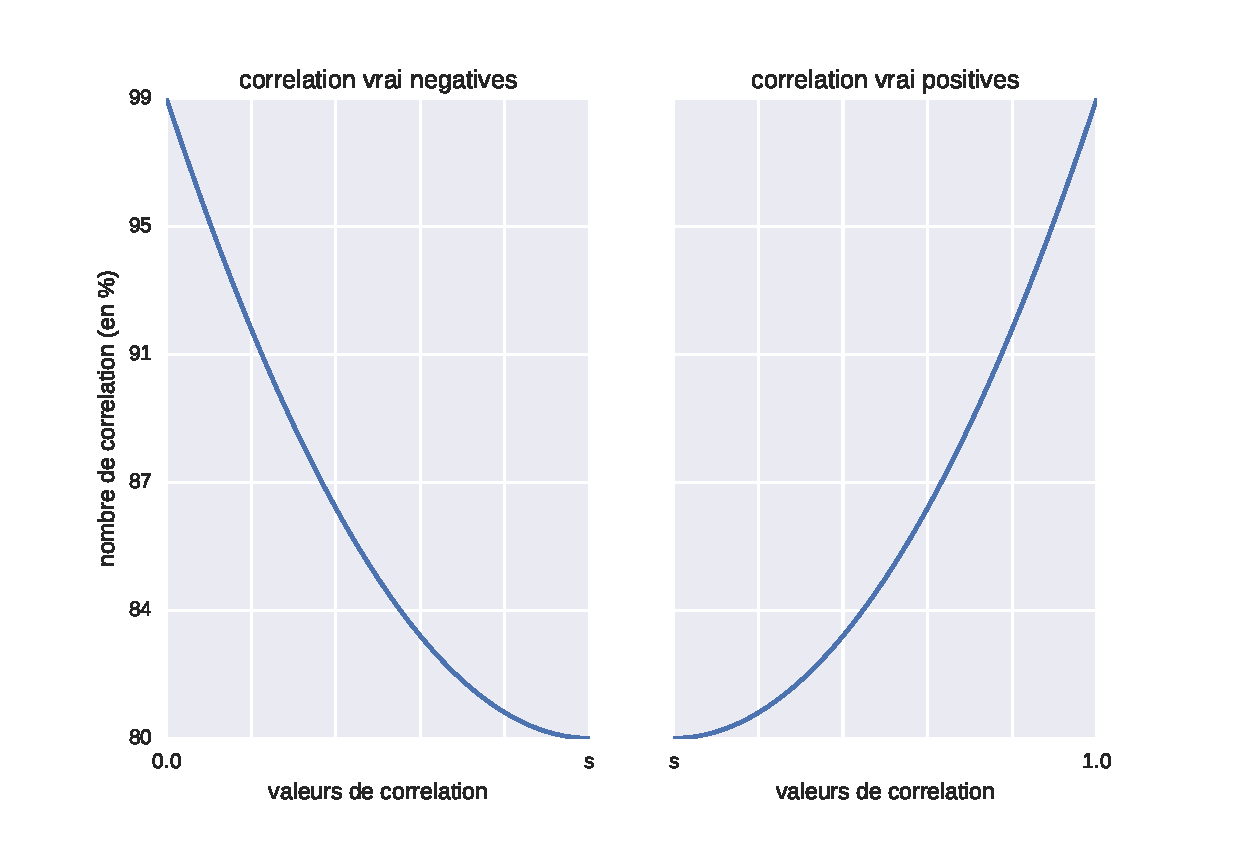
\includegraphics[scale=0.750]{vraiPositivesNegativesAutourDuSeuil.eps}
\caption{\`A gauche : Parabole croissante pour les erreurs {vrai positives} dans l'intervalle  $[s,1]$, \`a droite : Parabole d\'ecroissante pour les erreurs {vrai n\'egatives} dans l'intervalle $[0.s[$. L'ordonn\'e d\'esigne le taux de corr\'elation pour une valeur donn\'ee. }
\label{vraiPositivesNegativesAutourDuSeuil} 
\end{figure}
Cependant notre matrice $matE$ contient des erreurs de corr\'elations impliquant la pr\'esence de corr\'elations {\em fausses n\'egatives et fausses positives} autour de la valeur de seuil $p\_correl$ plutot que du seuil $s$. La variable $p\_correl$ est un seuil \`a partir duquel une corr\'elation est assez significative pour indiquer que deux ar\^etes partagent un sommet. En effet, le seuil $p\_correl$ est une valeur arbitraire choisie en fonction de l'hypoth\`ese de corr\'elation entre arcs (d\'efinition \ref{hypotheseCorrelationArcs}). 
\newline 
Ainsi, nous d\'efinissons quatre intervalles qui d\'esignent l'ensemble de valeurs pour les corr\'elations: 
\begin{itemize}
\item {\em vrai n\'egatives} $\rightarrow$ $int\_vn = [0, p\_correl - 0.2[$
\item {\em fausses n\'egatives} $\rightarrow$ $int\_fn = [p\_correl - 0.2, p\_correl[$
\item {\em fausse positives} $\rightarrow$ $int\_fp = [p\_correl, s[$
\item {\em vrai positives} $\rightarrow$ $int\_vp = [s, 1]$
\end{itemize}
Ainsi, les arcs adjacents ayant une corr\'elation comprise dans l'intervalle $int\_fn$ sont consider\'es comme {\em fausses n\'egatives} alors que pour une corr\'elation comprise dans l'intervalle $int\_fp$, les arcs non adjacents ont des corr\'elations {\em fausses positives}. 
Les intervalles sont resum\'es dans la figure \ref{intervallesFauxPositivesNegatives}.
Ainsi, si $p\_correl$ tend vers le seuil $s$, on a plus de corr\'elations {\em fausses n\'egatives} que des corr\'elations {\em fausses positives} dans la matrice $matE$. Par contre, le nombre de  corr\'elations {\em fausses positives} devient tr\`es \'elev\'e quand $p\_correl$ tend vers $0$.
\begin{centering} 
\begin{figure}[htb!] 
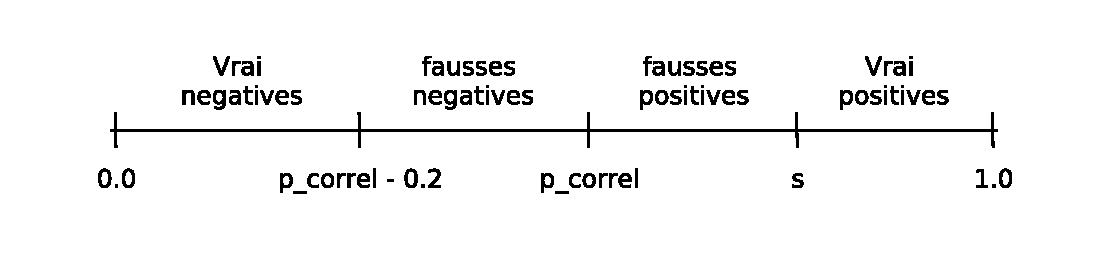
\includegraphics[scale=0.750]{intervallesFauxPositivesNegatives.eps}
\caption{ Correspondance entre valeurs et types de corr\'elations }
\label{intervallesFauxPositivesNegatives} 
\end{figure}
\end{centering} 
\newline
Nous retiendrons que les erreurs de corr\'elations se localisent autour du seuil $p\_correl$ et peuvent suivre diff\'erentes lois de probabilit\'es. La figure \ref{distributionErreursCorrelations} pr\'esente les courbes des distributions de corr\'elation. Les corr\'elations {\em fausses positives et fausses n\'egatives} suivent des lois normales %alors que celles {\em vrai positives et vrai n\'egatives} suivent des lois exponentielles de param\`etres $\lambda >1.5 $.
alors que celles {\em vrai positives} suivent des lois exponentielles de param\`etres $\lambda \ge 2$ et celles {\em vrai n\'egatives} avec des lois exponentielles invers\'ee avec $\lambda \le -2$.
\begin{centering} 
\begin{figure}[htb!] 
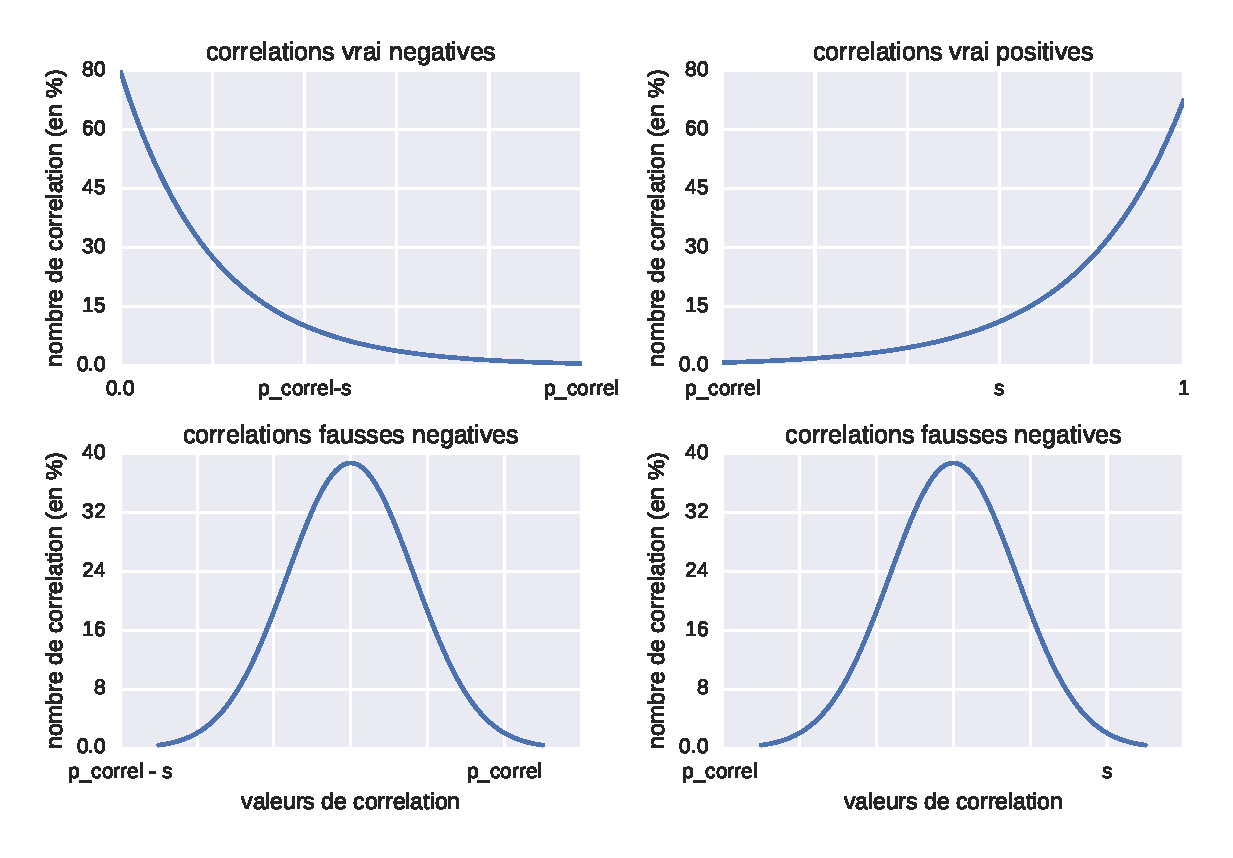
\includegraphics[scale=0.750]{distributionErreursCorrelations.eps}
\caption{En haut : loi exponentielle pour les erreurs   {\em vrai positives et vrai n\'egatives}, en bas : loi uniforme pour les erreurs   {\em fausses positives et fausses n\'egatives} }
\label{distributionErreursCorrelations} 
\end{figure}
\end{centering}  
\newline
L'utilisation de lois de probabilit\'e a pour but de montrer l'impact de seuil $p\_correl$ sur la line-couverture et aussi calculer les co\^uts de correction des sommets n'appartenant \`a aucune cliques.
%------  loi de distribution des correlation dans matE --> fin

%---- decription protocole d'etude --> debut
\subsection{Description du protocole d'\'etude}
% comment on va faire les etudes decrites plus haut 
% valeur du seuil  ==> ca se fera selon le distance line ???? je ne sais pas trop
% proposition de line-couverture : methodes de selection des sommets a -1
redecrire la partie en dessous et reprogrammer \newline
La r\'ealisation de notre \'etude passe par la g\'en\'eration de $500$ graphes de flots $G$ de $30$ sommets ayant un degr\'e maximal moyen $\Delta(G) = 5$ qui simulent le fonctionnement d'un r\'eseau \'electrique. Nous en d\'eduisons \'egalement $500$ line graphes de $150$ sommets et $470$ ar\^etes, en moyenne. \newline
Nous introduisons trois param\`etres $k, p\_correl, prob$:
\begin{enumerate}
\item $k$ d\'esigne le nombre de corr\'elations erron\'ees \`a ajouter dans la matrice $matE$. Dans notre \'etude, $k \in [1,9]$.
\item $p\_correl$ d\'esigne la probabilit\'e d'ajouter des erreurs de corr\'elations, soit corr\'elation {\em fausses positives} (ajout d'ar\^etes) soit corr\'elation {\em fausses n\'egatives} (suppression d'ar\^etes) soit les deux. Cette variable $p\_correl \in [0,1]$ varie par pas de $0.1$. Par exemple
	\begin{itemize}
	\item si $p\_correl=0$ $\rightarrow$ on a que des corr\'elations {\em fausses positives} dans la matrice $matE'$ car on supprime uniquement des ar\^etes dans le line graphe de matrice d'adjacence $matE$.
	\item si $p\_correl=0.5$ $\rightarrow$ le nombre de corr\'elations {\em fausses n\'egatives} et  {\em fausses positives} est approximativement semblable  dans la matrice $matE'$ car on ajoute et supprime \'equiprobablement des ar\^etes dans la matrice $matE$.
	\item si $p\_correl=1.0$ $\rightarrow$ la matrice $matE'$ ne contient que des corr\'elations {\em fausses n\'egatives} car on ajoute des ar\^etes dans le line graphe de matrice $matE$.
	\end{itemize}
\item $prob$ d\'esigne la probabilit\'e associ\'ee \`a une corr\'elation selon le type d'erreurs effectu\'e dans $matE'$. En un mot, $prob$ est la valeur de corr\'elation entre ar\^etes.
Ce param\`etre est important car les valeurs de corr\'elations calcul\'ees  ne sont pas binaires mais dependent d'une loi de probabilit\'e donc probabilistes. Nous en reparlerons \'egalement dans la section \ref{fonctionDeCout}.
\end{enumerate}
Pour ajouter des erreurs de corr\'elation \`a la matrice $matE$ correcte, on tire al\'eatoirement $k$ cases non encore modifi\'ees. Nous mettons chaque case et sa case sym\'etrique \`a $1$ si la probabilit\'e de la case est inf\'erieure ou \'egale \`a $p\_correl$. Si cette case est d\'ej\`a \`a $1$, on choisit une autre case. Selon le type d'erreurs de chaque case (vrai n\'egatives, vrai positives), on lui attribue une valeur de corr\'elation selon des distributions pr\'ed\'efinies.
\newline

Consid\'erons le graphe $G_k$ de matrice d'adjacence $matE_k$ dans laquelle on ajoute $k \in [1,9]$ erreurs de corr\'elation selon $p\_correl=0.5$, la probabilit\'e d'ajouter autant d'erreurs {\em fausses n\'egatives } et {\em fausses positives}. 
\`A la fin de l'ex\'ecution de l'algorithme de couverture, s'il existe des sommets de $G_k$ non couverts par {\em une ou deux cliques}, on les ajoute \`a l'ensemble des sommets \`a corriger $sommets\_1$ et nous appliquons l'algorithme  de correction sur chaque sommet de $sommets\_1$ selon les m\'ethodes suivantes:
\begin{itemize}
\item m\'ethode 1 : degr\'e minimum avec remise.\newline
Elle consiste \`a s\'electionner le sommet de degr\'e minimum dans l'ensemble $sommets\_1$, \`a appliquer l'algorithme de correction afin de modifier $matE$ et enfin \`a re-ex\'ecuter les deux algorithmes sur la matrice $matE$ modifi\'ee.
\item m\'ethode 2 : co\^ut minimum avec remise. \newline
Elle consiste \`a s\'electionner le sommet de co\^ut minimum dans l'ensemble $sommets\_1$, \`a appliquer l'algorithme de correction afin de modifier $matE$ et enfin \`a re-ex\'ecuter les deux algorithmes sur la matrice $matE$ modifi\'ee.
\item m\'ethode 3 : co\^ut minimum avec permutation des sommets de $sommets\_1$. \newline
Elle consiste \`a choisir une permutation dont les sommets sont class\'es par ordre croissant de leur co\^ut  de modification de la matrice $matE$ et \`a appliquer l'algorithme de correction sur cette permutation.
\item m\'ethode 4 :  degr\'e minimum avec  permutation des sommets de $sommets\_1$. \newline
Elle consiste \`a choisir une permutation dont les sommets sont class\'es par ordre croissant de leur degr\'e et \`a appliquer l'algorithme de correction sur cette permutation.
\item m\'ethode 5 : permutation al\'eatoire des sommets de $sommets\_1$. \newline
Elle consiste \`a choisir al\'eatoirement $N$ permutations puis \`a appliquer l'algorithme de correction et \`a s\'electionner la permutation ayant un co\^ut et une distance de Hamming minimum.
\end{itemize}

% calcul de moy_dl et moy_dh
Consid\'erons 
  $\alpha \in [1, 5]$ le nombre de fois qu'on applique $k$ erreurs dans la matrice $matE$ du line graphe $LG$,  
 $G_{k, \alpha}$ le graphe de matrice d'adjacence $matE_{k, \alpha}$ dont on a modifi\'e $k$ corr\'elations $\alpha$ fois et 
 $LG_{k, \alpha}$  le line graphe de matrice d'adjacence $matE_{k, \alpha}$ fourni par les algorithmes de couverture et de correction \`a partir du graphe $G_{k, \alpha}$.
\newline
En comparant
\begin{enumerate}
\item  $LG$ et $LG_{k, \alpha}$, on obtient la distance de Hamming not\'ee $DH_{k,\alpha}$.
\item $G_{k,\alpha}$ et $LG_{k,\alpha}$, on a la distance line not\'ee $DL_{k,\alpha}$.
\end{enumerate}
On d\'efinit par les variables $moy\_DH$ et $moy\_DL$, les moyennes respectives des distances de Hamming (not\'ee $DH_{k,\alpha}$) et des distances line (not\'ee $DL_{k,\alpha}$) pour une valeur donn\'ee de $k$ et pour tout $\alpha \in [1, 5]$.
\begin{equation}
moy\_DH_k = \sum_{\alpha = 1}^{5} DH_{k, \alpha} \hspace{2 em}
moy\_DL_k = \sum_{\alpha = 1}^{5} DL_{k, \alpha}
\end{equation}

Le protocole d'\'etude est recapitul\'e dans la figure \ref{recap_protocole_etude}. Le r\'eseau de flots $G$ g\'en\'er\'e est transform\'e en un line graphe $LG$, puis sont ajout\'es $k$ erreurs de corr\'elations $\alpha$ fois dans $LG$ pour obtenir $G_{k,\alpha}$. Nous appliquons les algorithmes (couverture et correction) pour determiner la line-couverture (ou la plus proche possible) du graphe $G_{k,\alpha}$ car ce graphe n'est pas n\'ecessairement un line graphe. Cette line-couverture correspond au line graphe $LG_{k, \alpha}$ qui est utilis\'e pour calculer les distances line ($DL_{k, \alpha}$) et de Hamming ($DH_{k, \alpha}$).
Les valeurs moyennes ($moy\_DL$, $moy\_DH$) des distances line et de Hamming sont calcules pour chaque erreur $k$ et leurs distributions sont pr\'esent\'ees dans la section suivante afin de monter les performances des algorithmes en pr\'esence d'erreurs de corr\'elations de diff\'erentes lois de probabilit\'es.
\begin{figure}[htb!] 
\centering
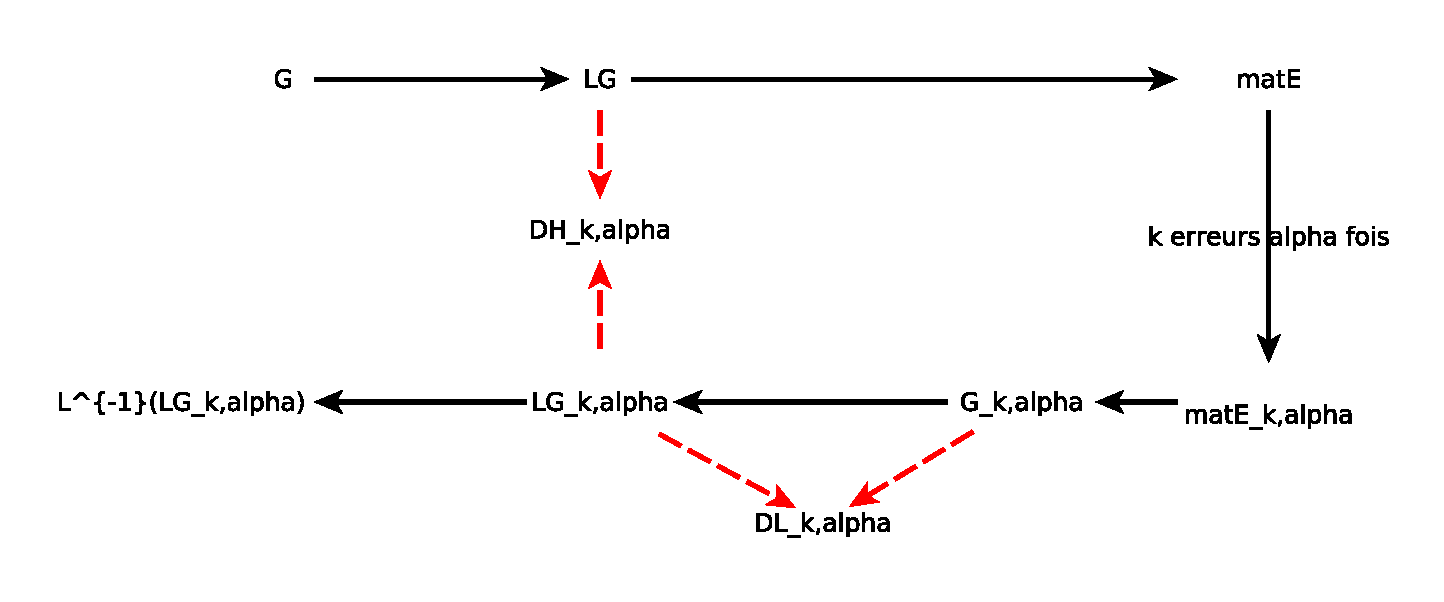
\includegraphics[scale=0.70]{recapProtocoleEtude.eps}
\caption{ Diff\'erentes \'etapes du processus de simulation de nos algorithmes (traits en noir), calcul de distances entre \'etapes}
\label{recap_protocole_etude} 
\end{figure}
%---- decription protocole d'etude --> fin
  
\section{Analyses et interpr\'etations}
Les valeurs de corr\'elations sont d\'efinies par les lois uniformes (erreurs vrai positives et vrai n\'egatives) et exponentielles (erreurs fausses positives et fausses n\'egatives) comme illustr\'e par la figure \ref{distributionErreursCorrelations} pour une probabilit\'e d'ajout des erreurs $p\_correl = 0.5$. Cela  signifie qu'il y a autant d'erreurs fausses positives que d'erreurs fausses n\'egatives dans la matrice de corr\'elation du graphe $G_{k}$. Ces lois de distribution respectent l'hypoth\`ese de corr\'elations des arcs (voir la d\'efinition \ref{hypotheseCorrelationArcs}). 
\newline
% interpretation d'une distribution  DH et DL pour une methode
% presentation des differentes methodes et comparaison
% comparaison entre differentes p
% impact de la fonction de cout
Nous d\'ecrirons d'abord les distributions des distances line et de Hamming moyenn\'ees ($moy\_DL$ ou $moy\_DH$) pour une m\'ethode de correction (al\'eatoire). Ensuite nous comparons les cinq m\'ethodes de correction en nous basant sur les distances de Hamming moyenn\'ees. 
Enfin nous expliquons le choix de la m\'ethode de {\em permutation al\'eatoire} et montrons que les algorithmes (couverture et correction) proposent de meilleurs r\'esultats lorsque la matrice de corr\'elation poss\`ede plus de corr\'elations {\em faux n\'egatives} que de corr\'elations {\em faux positives} et aussi peu d'erreurs de corr\'elations ($k < 6$). 
\newline
Nous pr\'esentons \'egalement l'impact de la fonction de co\^ut dans les distributions  de distances de Hamming et 
la relation existance entre la distance line et la distance de Hamming.

\subsection{Distribution de la m\'ethode de permutation al\'eatoire}
% description distribution methode aleatoire
% expliquer les distributions moy_dh et moy_dl  et les courbes de ces distributions pour une methode de correction
% interpretation selon loi uniforme  pour p = 0.5
% k = [0,5] : une figure
% k = [6,9] : une autre figure
% k = [10,50] : une autre figure
% cas particulier pour la loi de poisson
\begin{figure}[htb!] 
\centering
%\includegraphics[scale=0.150]{permut_distanceMoyenDLDH_k_0_4_aleatoire_p_05.jpeg}
\includegraphics[width=550pt, height=600pt]{permut_distanceMoyenDLDH_k_0_4_aleatoire_p_05.jpeg}
\caption{ M\'ethode de permutation al\'eatoire avec une fonction de correction \`a co\^ut unitaire : distribution des distances line $moy\_DL$ et de Hamming $moy\_DH$ pour $k \in [0,  5]$ corr\'elations alter\'ees}
\label{permut_distanceMoyenDLDH_k_0_5_aleatoire_p_05} 
\end{figure}

\begin{figure}[htb!] 
\centering
\includegraphics[width=550pt,height=600pt]{permut_distanceMoyenDLDH_k_5_9_aleatoire_p_05.jpeg}
\caption{ M\'ethode de permutation al\'eatoire avec une fonction de correction \`a co\^ut unitaire : distribution des distances line $moy\_DL$ et de Hamming $moy\_DH$ pour $k \in [6,  9]$ corr\'elations alter\'ees}
\label{permut_distanceMoyenDLDH_k_5_9_aleatoire_p_05} 
\end{figure}


La figure \ref{permut_distanceMoyenDLDH_k_0_5_aleatoire_p_05} repr\'esente les distributions des distances line, de Hamming, des fonctions de r\'epartition de la corr\'elation entre distances line et Hamming pour $k \in [0,5]$ erreurs. \newline
Pour $k=0$ erreur, nous avons un batonnet sur les histogrammes de distances line et de Hamming. Ce batonnet est le pourcentage d'ar\^etes identiques entre les graphes $G_k$ et $LG_k$ (distance line) et aussi entre les graphes  $LG$ et $LG_k$. Nous constatons que  le pourcentage est de $100\%$ impliquant que les ar\^etes des graphes $LG_k$, d\'ecouvertes par les algorithmes, sont identiques \`a celle du graphe $LG$. Ce qui est normal parce que nous n'avons ajout\'e aucune erreur dans le line graphe $LG$. Les courbes des fonctions de r\'epartition  suivent l'\'equation \ref{eqCorrelMoyDLDH} pour la corr\'elation entre les distances line et de Hamming et l'\'equation \ref{eqCumulMoyDH} pour la distance de Hamming.
\begin{equation}
\label{eqCorrelMoyDLDH}
y = \left\{
	\begin{aligned}
	0 \hspace{1 em} si \hspace{1 em} x < 1 \\
	100  \hspace{1 em}  si  \hspace{1 em}  x = 1
	\end{aligned}
	\right.
\end{equation}
\begin{equation}
\label{eqCumulMoyDH}
y = 1  \hspace{1 em}  si  \hspace{1 em}   x \in [0,1]
\end{equation}
Nous nous servirons du cas de $k=0$ erreur comme une r\'ef\'erence de la meilleure performance de nos algorithmes.
\newline
Pour $k \in [1,4]$, l'ensemble des batonnets, regroup\'es avant la droite $y = k$ (droite en rouge) de chaque histogramme, a un pourcentage sup\'erieure \`a $50 \%$. La pr\'esence de cette droite nous indique que, dans le majorit\'e des cas,  qu'il existe une diff\'erence de $k$ ar\^etes entre les graphes $G_k$ et $LG_k$ (voir distance line figure \ref{permut_distanceMoyenDLDH_k_0_5_aleatoire_p_05}) et ces $k$ ar\^etes correspondent aux erreurs ajout\'ees dans la matrice d'adjacence $matE$ du line graphe $LG$. Cela explique 
la distance de hamming de $0$ ar\^ete entre $LG$ et $LG_k$ et le pourcentage pour $0$ erreur est le pic de chaque histogramme (voir distance de Hamming figure \ref{permut_distanceMoyenDLDH_k_0_5_aleatoire_p_05}).
% ajouter les fonctions cumulatives

Au d\'el\`a de $k \ge 5$ erreurs, le pic de chaque histogramme baisse significativement quand $k$ augmente (voir distances line et de  Hamming figure \ref{permut_distanceMoyenDLDH_k_5_9_aleatoire_p_05}). Une explication est la pr\'esence d'ar\^etes erron\'ees dans les line graphes $LG_k$ propos\'es parce que la majorit\'e de ces line graphes qui ont plus de $k$ ar\^etes diff\'erentes entre $LG_k$ et $G_k$ alors que ce nombre $k$ doit correspondre au nombre d'erreurs ajout\'ees dans le line graphe $LG$. Il s'illustre parfaitement avec $k = 9$ erreurs dans la figure \ref{permut_distanceMoyenDLDH_k_5_9_aleatoire_p_05} o\`u on a moins de $13\%$ de line graphes dont les ar\^etes sont identiques et les $87\%$ restants ont plus d'une  ar\^ete diff\'erente.
\newline
%-------
Par ailleurs, les fonctions de r\'epartition des corr\'elations entre distances line et de Hamming et celle de la distance de Hamming ont des courbes  qui s'eloignent de celle de $k = 0$ erreur. En effet, ces courbes se divisent en deux parties : une courbe croissante et une droite verticale (distance de Hamming) ou horizontale (distance line). 
Pour $k \in [1,4]$, dans les figures des distributions cumulatives des distances de Hamming (colonne 4 de la figure \ref{permut_distanceMoyenDLDH_k_5_9_aleatoire_p_05}), on remarque que la droite verticale pour $k$ erreurs baisse quand $k$ augmente. Cette droite est le pourcentage de line graphes identiques ($LG$ et $LG_k$). Par exemple, on a $69\%$ de line graphes $LG_k$ identiques \`a $LG$ pour $k = 1$ alors qu'on en a que $19\%$ pour $k=4$. Cela est d\^u \`a l'ajout d'ar\^etes dans $LG_k$ n'appartenant pas \`a $LG$. Cela  forme une courbe exponentielle croissante dans laquelle on a plus de $10$ ar\^etes diff\'erentes pour $k \le 5$.  \newline
De m\^eme, au d\'el\`a du nombre ar\^etes diff\'erentes c'est-\`a-dire $moy\_DH > k$, nous constatons une droite verticale tr\`es courte qui baisse \'egalement quand la variable $moy\_DH$ augmente. Cela signifie qu'il y a tr\`es peu de line graphes $LG_k$ ayant des  distances de Hamming tr\`es \'elev\'ees par rapport aux $k$ erreurs (voir figures \ref{permut_distanceMoyenDLDH_k_0_5_aleatoire_p_05} et \ref{permut_distanceMoyenDLDH_k_5_9_aleatoire_p_05})  pour $k \ge 5$.
\newline
Le fait que les distributions de distance line et de Hamming soient, toutes les deux, asym\'etriques (pour $k \le 6$) soient sym\'etriques (pour $k>6$) nous interrogent sur l'\'evolution des distributions des distances line par rapport \`a celles de Hamming. 
%Les colonnes $3$ des figures\ref{permut_distanceMoyenDLDH_k_0_5_aleatoire_p_05} et \ref{permut_distanceMoyenDLDH_k_5_9_aleatoire_p_05} presentent les corr\'elations entre distances line et de Hamming moyenn\'ees  elles evoluent identiquement que celle de Hamming 



%\begin{centering} 
%\begin{figure}[htb!] 
%\includegraphics[scale=0.10]{permut_aleatoire_coutMin_degreMin_fct_cout_unitaire_500G/aleatoire/courbes/distanceMoyenDLDH_k_0_10_aleatoire_p_05.jpeg}
%\caption{ M\'ethode permutation al\'eatoire avec co\^ut unitaire : distribution des distances line $moy\_DL$ et de Hamming $moy\_DH$ pour $k \in [1,  9]$ corr\'elations alter\'ees}
%\label{distLineHammingPermutAleatoireK09p05} 
%\end{figure}
%\end{centering} 
%\begin{centering} 
%\begin{figure}[htb!] 
%\includegraphics[scale=0.09]{/home/willy/Documents/courbePython/courbeDegreCoutMinAleatoire_11_09_2017/permut_aleatoire_coutMin_degreMin_fct_cout_unitaire_500G/aleatoire/courbes/repartition_corr\'elation_k_0_10_aleatoire_p_05_2D.jpeg}
%\caption{ M\'ethode co\^ut minimum avec remise : fonction de repartition cumul\'ee des distances line $moy\_DL$ et de Hamming $moy\_DH$ pour $k \in [1, \cdots, 9]$ de corr\'elations alter\'ees}
%\label{fctRepartitionCumuleDistLineHammingPermutAleatoireK09p05} 
%\end{figure}
%\end{centering} 
%La figure \ref{distLineHammingPermutAleatoireK09p05} repr\'esente les histogrammes de la m\'ethode de permutation al\'eatoire pour une probabilit\'e $p=0.5$ et une fonction de co\^ut normale $F_1$. \`A gauche de cette figure, nous avons les distributions des distances lines et \`a droite celle des distances de Hamming. Ces histogrammes partent d'une corr\'elation modifi\'ee (en haut de la figure \ref{distLineHammingPermutAleatoireK09p05}) \`a $9$ corr\'elations  modifi\'ees (en bas de la figure \ref{distLineHammingPermutAleatoireK09p05}). 
%\newline
%Dans la repr\'esentation d'une distribution, chaque batonnet correspond au pourcentage de graphes associ\'e \`a une distance moyenn\'ee (line ou Hamming).
%\`A titre d'exemple, pour $k=2$ corr\'elations modifi\'ees, le pic de l'histogramme est \`a $moy\_DL = 2$ pour les distances lines et de $moy\_DH=0$ pour les distances de Hamming. 
%Les pourcentages de graphes pour  $moy\_DL = 2$ et $moy\_DH=0$ sont identiques c'est-\`a-dire $50\%$. 
%Ce resultat s'explique par la modification des ar\^etes associ\'ee aux $k = 2$ corr\'elations erron\'ees impliquant la d\'ecouverte du line graphe du r\'eseau de flots.
%Par ailleurs, pour $k = 9$ corr\'elations \'erron\'ees, le pourcentage de line graphes fournis $LG_{k,\alpha}$ correspondant aux line graphes $LG$ des r\'eseaux de flots pour $moy\_DL = 9$ et $moy\_DH=0$ est de $1\%$. 
%En plus, le pourcentage de line graphes associ\'e au pic de l'histogramme i.e $moy\_DH = 20$ est de $5\%$.
%L'algorithme de line graphes donne de mauvais r\'esultats pour $k=9$ errors de corr\'elations.
%\newline
%Nous avons, dans les histogrammes, une droite verticale $y = k$ (en rouge) correspondant \`a $k$ erreurs de corr\'elations.
%On constate que les pics sont \`a gauche sur la droite $y = k$ pour $k \le 6$ corr\'elations modifi\'ees.
%Cela signifie que le pourcentage de graphe dont $moy\_DL = k$  et $moy\_DH=0$ est le plus \'elev\'e (on retrouve en g\'en\'eral le line graphe initial $LG$) entrainant une asym\'etrie vers la droite de la distribution des distances pour $k \le 6$.
%En revanche, au d\'el\`a de $k>6$, l'algorithme de correction retrouve peu de corr\'elations modifi\'ees. Ce qui place le pic ($moy\_DL$ ou $moy\_DH$) \`a droite de la droite $y = k$ et fournit une distribution gaussienne des distributions. \newline
%Le fait que les distributions de distance line et de Hamming soient, toutes les deux, asym\'etriques (pour $k \le 6$) soient sym\'etriques (pour $k>6$) nous interrogent sur l'\'evolution des distributions de distance line par rapport \`a celle de Hamming. 
% Pour cela, on calcule leur corr\'elation par la fonction $F$ d\'efinie en \ref{formuleCorrelation} et dont la fonction de r\'epartition cumul\'ee est dans la figure \ref{fctRepartitionCumuleDistLineHammingPermutAleatoireK09p05}.
%\begin{equation}
%\label{formuleCorrelation}
%F_{k, \alpha} = \frac{ | moy\_DL_{k, \alpha} - moy\_DH_{k, \alpha} | }{ max(moy\_DL_{k, \alpha},  moy\_DH_{k, \alpha}) }
%\end{equation}
%Si $moy\_DL$ et $moy\_DH$ \'evoluent de mani\`ere oppos\'e (l'un est sup\'erieur \`a $0$, l'autre est \'egal \`a $0$), la fonction $F$ est \'egale \`a $1$. Par contre, s'ils sont tr\`es corr\'el\'es (i.e \'evoluent identiquement) alors $F = 0$.
%Ainsi lorsqu'elles \'evoluent dans le m\^eme ordre, on obtient la courbe racine carr\'ee. Tel est le cas dans la figure \ref{fctRepartitionCumuleDistLineHammingPermutAleatoireK09p05} pour $k > 6$. 
%Les courbes tendent vers la fonction racine carr\'ee quand $k$ devient grand. 
%Par ailleurs $F \approx 0$ quand $k$ est tr\`es petit (fig \ref{fctRepartitionCumuleDistLineHammingPermutAleatoireK09p05}, $k \le 6$).
%\newline

% relation entre DL et DH
\subsection{Relation entre la distance line et la distance de Hamming}
Les r\'eseaux r\'eelles, dont nous poss\'edons les mesures de flots sur les arcs, sont inconnus.
Cela implique que la distance de Hamming est impossible \`a d\'eterminer.
\'Etant donn\'ee que nous avons le line graphe $G_{k,\alpha}$ du r\'eseau de flots dans nos simulations, nous pouvons calculer les distances de Hamming et line. 
\newline
La distance line est la distance de Hamming minimum entre $LG$ et $LG_{k,\alpha}$ pendant la correction des sommets. 
Elle compare les line graphes obtenus $LG_{k,\alpha}$ apr\'es correction du graphe $G_{k,\alpha}$ pour en fournir un line graphe dont la correction des sommets est de co\^ut minimum.
\newline
Nous calculons la corr\'elation entre les distances line et de Hamming \`a partir de la formule \ref{correlation_line_hamming}.
%\begin{multline}
\begin{equation}
	corr_{k,\alpha} =  \frac{ | moy\_DL_{k, \alpha} - moy\_DH_{k, \alpha} | }{ max(moy\_DL_{k, \alpha},  moy\_DH_{k, \alpha}) };
	\\
	corr_{k} = \sum_{\alpha = 1}^{5}corr_{k,\alpha} ;
	\\
	F_k (x) = P(corr_{k} \le x ) 
\label{correlation_line_hamming}
\end{equation}
%\end{multline}
avec $x \in [0,1]$ une valeur de corr\'elation et $k$ le nombre d'erreurs de corr\'elation. 
\newline
Sur la figure \ref{dh_vs_dl_p_05}, est repr\'esent\'e la fonction de repartition $F_k$ dans laquelle nous avons, en absicce, la corr\'elation entre les distances et, en ordonn\'e, le pourcentage de graphes dont la corr\'elation $corr$ est inf\'erieure \`a $x$. 
\begin{figure}[htb!] 
\centering
\includegraphics[scale=0.35]{comparaison_entre_fct_cout_et_methodes_correction/correlation_dh_dl_p_05.jpeg}
\caption{ distance line versus distance de Hamming pour $k$ erreurs de corr\'elation et $p = 0.5$ }
\label{dh_vs_dl_p_05} 
\end{figure}
En effet si $corr_k = 1$ alors il n'existe aucune corr\'elation entre les distances line et de Hamming. Cela signifie que le line graphe fourni $LG_{k}$ est  le veritable line graphe de $LG$ sur notre r\'eseau de flots $G$ ($LG_{k} = LG$). 
De m\^eme, si $corr_k = 0$ alors les distances line et de Hamming sont identiques. Cela signifie que ajouter/supprimer ces ar\^etes au line graphe $LG_k$ produit le line graphe de notre r\'eseau ($LG_{k} \neq LG$) et que $LG_{k}$ et $LG$ sont differents de $k$ ar\^etes quand $k < 6$.
\newline
Donc si $F_k(1) \approx 0$ alors le nombre de corr\'elation $corr_k = 1$ est tr\`es \'elev\'e. Cela s'illustre sur la figure \ref{dh_vs_dl_p_05} par les courbes de $k=[2,5]$. 
Par exemple $F_5(1) \approx 10\%$ signifie que nous avons $70-10=60\%$ line graphes $LG_k$ correspondant aux line graphes $LG$ des r\'eseaux. ($corr_5 \approx 60\%$ et $70\%$ le pourcentage de corr\'elations \'egale \`a $1$).
\newline
Par compte, si  $F_k(1)$ est tr\`es \'elev\'e, cela signifie que le nombre de $corr_k = 1$ est tr\`es faible entrainant une corr\'elation tr\`es forte en les distances line et de Hamming.
C'est notre constat avec les courbes de $k = [10,20]$ dans lesquelles nous avons une  croissante continue en fonction de l'augmentation des valeurs de corr\'elations.
\newline
Nous subdivisons nos courbes en deux cat\'egories:
\begin{itemize}
	\item Celle dont on a une corr\'elation entre distances lines et de Hamming (courbes de $k = [10,20]$).
	\item celle dont on a aucune corr\'elation entre ces distances parce que nous fournissons le line graphe du r\'eseau c'est-\`a-dire  $LG = LG_k$ (courbes de $k = [2,5]$). 
\end{itemize}
Nous pouvons conclure que l'utilisation de la distance line est une bonne m\'etrique pour juger de la qualit\'e de notre algorithme de correction en absence de la distance de Hamming parce que une distance line inf\'erieure \`a $5$ fournit le line graphe $LG$ du r\'eseau de flots tandis qu'une distance sup\'erieure \`a $10$ correspond au nombre de corr\'elations \`a modifier pour delivrer le line graphe $LG$. 

\subsection{Comparaison des m\'ethodes de correction}
% comparer les differentes methodes selon la description sur la methode aleatoire
Nous recherchons la meilleure m\'ethode de correction parmi les cinq m\'ethodes \'enumer\'ees plus haut. 
Pour ce faire, on dispose des distributions de distances line et de Hamming, des histogrammes, des fonctions de repartitions de ces distributions et aussi des moyennes de distances line/Hamming associ\'ees \`a $k$ corr\'elations \'erron\'ees pour chacune des m\'ethodes regroup\'ees dans les figures \ref{permut_distanceMoyenDLDH_k_0_5_aleatoire_p_05} et \ref{permut_distanceMoyenDLDH_k_5_9_aleatoire_p_05}.  
Nous utilisons la moyenne des distances de Hamming pour la comparaison de m\'ethodes parce que la distance de Hamming permet d'\'evaluer la diff\'erence entre le graphe de base $LG$ et celui pr\'edit $LG_k$ par nos algorithmes et aussi nous connaissons les line graphes associ\'es aux r\'eseaux \'electriques.\newline
Rappelons que nous avons la probabilit\'e $p\_correl=0.5$ et la fonction de co\^ut est unitaire ($F_0$).
La figure \ref{compareDifferentesMethodesCorrectionSommets_fct_cout_unitaire_p05} affiche les courbes  des diff\'erentes m\'ethodes pour des distances de Hamming moyenn\'ees en fonction des $k$ erreurs de corr\'elations.
\newline
Nous constatons  que la pire des m\'ethodes est celle de degr\'e minimum avec remise (en rouge avec un rond) car elle est au dessus des autres et la meilleure est celle de {\em de permutation al\'eatoire} (en jaune avec un triangle) car elle propose des line graphes ayant  le nombre minimum d'ar\^etes diff\'erentes pour $ \forall k$.\newline
\begin{figure}[htb!] 
\centering
% a changer par des chemins relatifs
\includegraphics[scale=0.25]{comparaison_MethodesCorrection_fctDeCout_permut_aleatoire_coutMin_degreMin/comparaisonDifferentesMethodesFonctDeCout_normal_500G_p_05.jpeg}
\caption{ Comparaison des diff\'erentes m\'ethodes de correction de sommets pour $k \in [1,9]$ corr\'elations modifi\'ees. Les courbes en bleu carr\'e, rouge carr\'ee, rouge rond, vert rond et jaune triangle sont associ\'ees respectivement aux m\'ethodes 1, 2, 3, 5, 4 }
\label{compareDifferentesMethodesCorrectionSommets_fct_cout_unitaire_p05} 
\end{figure}
Nous retenons, pour la suite, la m\'ethode de {\bf permutation al\'eatoire} comme m\'ethode de correction des sommets n'appartenant \`a aucune couverture (sommets $\in sommets\_1$).
\newline


\subsection{Influence des erreurs de corr\'elations sur les distributions}
% comparaison de p sur la methode de permutation aleatoire
\begin{figure}[htb!] 
\centering
% meilleur probabilite p parmi les [0.0, 0.1, 0.2, ...., 1.0]
% a changer par des chemins relatifs
\includegraphics[scale=0.25]{permut_aleatoire_coutMin_degreMin_fct_cout_normal_500G/aleatoire/courbes/comparaison_probabilities_p_00_10_moy_dh_aleatoire_p_10.jpeg}
\caption{ Comparaison des diff\'erentes probabilit\'es d'ajout $k \in [1,9]$ de corr\'elations fausses positives et fausses n\'egatives sur la m\'ethode de permutation al\'eatoire }
\label{compareDifferentesProbabilitesP0_1_fct_cout_unitaire_p05} 
\end{figure}

%------ a effacer cette image --------%
%\begin{centering} 
%\begin{figure}[htb!] 
%% distribution de p = 1.0 
%% a changer par des chemins relatifs
%\includegraphics[scale=0.10]{permut_aleatoire_coutMin_degreMin_fct_cout_normal_500G/aleatoire/courbes/distanceMoyenDLDH_k_0_10_aleatoire_p_10.jpeg}
%\caption{ distribution des distances line et de Hamming pour $p=1.0$ et $k \in [1,9]$ corr\'elations modifi\'ees}
%\label{distributionDLDH_p1.0_k19_fct_cout_unitaire} 
%\end{figure}
%\end{centering} 
%------ a effacer cette image --------%

Faisons varier la variable $p\_correl \in [0,1]$ par pas de $0.1$ dans le but de visualiser l'impact de corr\'elations {\em fausses positives} et {\em fausses n\'egatives} dans l'ex\'ecution des algorithmes. Rappelons que l'ajout et la suppression d'ar\^etes ont le m\^eme co\^ut de traitement c'est-\`a-dire $1$.
La figure \ref{compareDifferentesProbabilitesP0_1_fct_cout_unitaire_p05} r\'esume l'\'evolution des types d'erreurs de corr\'elations ($p\_correl$) pour des distances de Hamming $moy\_DH$ en fonction de  $k \in [1, 9]$  erreurs de corr\'elations.
\newline 
Nous constatons que les algorithmes donnent de meilleurs r\'esultats pour $p\_correl = 1$ et de mauvais r\'esultats pour $p\_correl = 0$. 
En d'autres termes, lorsqu'on ajoute que des corr\'elations {\em fausses n\'egatives} i.e $p\_correl  = 1$ dans la matrice $matE$, les algorithmes  proposent, dans la majorit\'e des cas, un line graphe $LG_k$ dont ces erreurs de corr\'elation sont supprim\'ees. Cela s'illustre dans la figure \ref{permut_distanceMoyenDLDH_k_5_9_aleatoire_p_10} o\`u l'ajout de $5$ corr\'elations {\em fausses n\'egatives} influencent tr\`es peu les line graphes propos\'es $LG_{k}$ puisqu'ils sont identiques aux line graphes initiales $LG$ dans $45\%$ des cas. 
En revanche, ce pourcentage baisse avec beaucoup d'erreurs de corr\'elations. Tel est le cas pour $k = 9$ corr\'elations o\`u le taux est de $24\%$. 
\begin{figure}[htb!] 
\centering
%\includegraphics[width=550pt,height=600pt]{permut_distanceMoyenDLDH_k_5_9_aleatoire_p_10.jpeg}
\caption{ M\'ethode de permutation al\'eatoire avec une fonction de correction \`a co\^ut unitaire et $p\_correl = 1.0$ : distribution des distances line $moy\_DL$ et de Hamming $moy\_DH$ pour $k \in [6,  9]$ corr\'elations alter\'ees}
\label{permut_distanceMoyenDLDH_k_5_9_aleatoire_p_10} 
\end{figure}
%En revanche, ce pourcentage baisse malgr\'e le nombre \'elev\'e de corr\'elations {\em fausses positives}. Tel est le cas pour $k = 9$ corr\'elations o\`u le taux est de $24\%$. 
\newline
Par ailleurs, le mauvais r\'esultat obtenu pour des probabilit\'es $p < 0.5$ s'explique par le mode de fonctionnement de l'algorithme de correction. En Effet, cet algorithme consiste \`a ajouter des ar\^etes au voisinage du sommet \`a corriger puis de supprimer certaines ar\^etes pour \'eviter qu'un sommet n'appartienne \`a plus de $2$ cliques (propriet\'e du line graphe).
\newline
Nous pensons que le meilleur compromis est la probabilit\'e $p\_correl = 0.7$ parce que, pour peu de corr\'elations modifi\'ees ($k<5$), les lines graphes produits $LG_k$ et g\'en\'er\'es $LG$ diff\`erent de $k<6$ ar\^etes correspondant aux $k$ erreurs de  corr\'elations \'effectu\'ees  et au d\'el\`a $k \geq 6$, le nombre d'ar\^etes diff\'erentes est fonction du nombre de corr\'elations faites multipl\'e par $1.5$.
Cela signifie qu'il faut, dans la matrice de corr\'elation, $30\%$ de corr\'elations {\em fausses positives} et $70\%$ de corr\'elation {\em fausses n\'egatives}. 
\newline
%Que se passe-t-il si on priorise l'ajout de corr\'elations {\em fausses n\'egatives} \`a chaque traitement c'est-\`a-dire la suppression d'ar\^etes?  
%En d'autres termes, l'ajout d'ar\^etes {\em fausses positives} a un co\^ut moins important que celui des {\em fausses n\'egatives}. 
%----
Que se passe-t-il si on priorise l'ajout de corr\'elations {\em fausses positives} \`a chaque traitement c'est-\`a-dire l'ajout d'ar\^etes?  
En d'autres termes, la suppression d'ar\^etes {\em fausses n\'egatives} a un co\^ut moins important que celui des {\em fausses positives}. 
%----

%Le co\^ut de traitement d'un sommet a-t-il un impact sur le graphe propos\'e?
\subsection{Impact de la fonction de co\^ut sur les distributions}
% urgent definir les fourchettes de probas pour chaque type de corr\'elation
\label{fonctionDeCout}

\begin{figure}[htb!] 
\centering
% a changer par des chemins relatifs
\includegraphics[scale=0.25]{comparaison_MethodesCorrection_fctDeCout_permut_aleatoire_coutMin_degreMin/comparaisonDifferentesFonctDeCout_by_permut_aleatoire_p_05.jpeg}
\caption{ Comparaison des diff\'erentes fonctions de co\^ut avec l'ajout de $k \in [1,9]$ de corr\'elations fausses positives et fausses n\'egatives pour une probabilit\'e $p = 0.5$ avec la m\'ethode de permutation al\'eatoire }
\label{compareDifferentesFonctionDeCout_p05} 
\end{figure}

Nous d\'efinissons quatre fonctions de co\^ut: unitaire (n=0), normal (n=1), quadratique (n=2), puissance 4 (n = 4) selon l'expression suivante
\begin{equation}
	\begin{aligned}
	F_n = 
	\begin{cases}
		prob[(a_i,a_j)]^n   \\
		(1 - prob[(a_i,a_j)])^n \\
	\end{cases}
	\end{aligned}
\end{equation}
ou $prob[(a_i,a_j)]^n$, la corr\'elation entre les ar\^etes $a_i$ et $a_j$, correspondant au co\^ut d'ajout de corr\'elations fausses n\'egatives, 
$(1-prob[(a_i,a_j)])^n$ au co\^ut d'ajout de corr\'elations fausses positives.
\newline
\'Etant donn\'ee que nous avons utilis\'e des matrices binaires dans la g\'en\'eration de line graphes, nous assignons des probabilit\'es pour chaque type de corr\'elation tel que:
\begin{itemize}
\item $prob[(a_i,a_j)] = [0, 0.5[ $ : corr\'elation vrai n\'egative i.e $0 \rightarrow 0$
\item $prob[(a_i,a_j)] = [0.5, 0.79[ $: corr\'elation fausse n\'egative i.e $1 \rightarrow 0$
\item $prob[(a_i,a_j)] = 0.8 $ : corr\'elation fausse positive i.e $0 \rightarrow 1$
\item $prob[(a_i,a_j)] = ]0.8, 1] $ : corr\'elation vrai positive i.e $1 \rightarrow 1$
\end{itemize}
La figure \ref{compareDifferentesFonctionDeCout_p05} affiche les courbes des diff\'erentes fonctions de co\^ut selon les $k$ corr\'elations modifi\'ees pour $p\_correl = 0.5$.
\newline
Les $4$ courbes sont superpos\'ees pour $k\le5$ et au d\'el\`a de $k>5$, les courbes carr\'ee (n=2) et normal (n=1) ont les plus petites distances moyenn\'ees de Hamming.
Pour $k>9$, la courbe unitaire (n=0) \'evolue de mani\`ere exponentielle tandis que les courbes quadratique (n=2) et normal (n=1) ont un rapport de $2$ entre les distances de Hamming et le nombre $k$ de corr\'elations modifi\'ees.
On en d\'eduit que la pire fonction de co\^ut est la fonction unitaire (n=0 en jaune).
\newline
Cependant, nous ne pouvons pas choisir la meilleure fonction de co\^ut car les fonctions des courbes {\em normal} et {\em quadratique} \'evoluent identiquement.
 On peut conclure qu'utiliser les probabilit\'es de corr\'elations pour le calcul du co\^ut am\'eliore significativement les distances moyenn\'ees de Hamming.
 \newline
 On choisit pour la suite la fonction de co\^ut normal $F_1$ pour le co\^ut de modification de chaque ar\^ete. 

\subsubsection{Cas particulier: fonction de co\^ut en cloche}
%petit rappel sur comment fonctionne la correction avec les autres fonctions de cout
Souvenons nous que corriger la matrice binaire de corr\'elation consiste \`a modifier les cases de cette matrice par leurs valeurs contraires.
Le cas id\'eal serait la modification des corr\'elations fausses positives et fausses n\'egatives pendant la phase de correction.
Cependant, pendant cette phase, la correction est effectu\'ee autant sur les corr\'elations fausses positives et fausses n\'egatives que sur celles vrai positives et vrai n\'egatives.
L'algorithme de correction ne fait aucune distintion entre les corr\'elations fausses et les bonnes corr\'elations.
Afin de prioriser la modification des corr\'elations fausses, nous definisons une nouvelle fonction de co\^ut appel\'ee {\em cloche}.
\newline
% definir la fonction de cloche et sa particularite
La fonction {\em cloche} se d\'efinit ainsi:
\begin{equation}
	F_c = | 4\cdot((p-s) - (s-0.5))^2 |^{1.5}  
\end{equation}
La fonction de co\^ut cloche est une fonction polynomiale de degr\'e $2$ qui applique des poids aux ar\^etes de sorte que les ar\^etes, dont les corr\'elations avoisinent le seuil, sont moins p\'enalis\'ees et les ar\^etes, dont les corr\'elations sont \'eloign\'ees du seuil, ne sont quasi jamais utilis\'ees pendant la phase de correction. 
Les poids minimaux sont appliqu\'es pour les corr\'elations fausses tandis que les poids maximaux (= $1$) sont appliqu\'es aux bonnes corr\'elations
%La fonction de co\^ut cloche est une fonction polynomiale de degr\'e $2$ qui applique les co\^uts les plus \'elev\'es aux corr\'elations exactes (c'est-\`a-dire $1$) et les co\^uts les plus faibles aux corr\'elations fausses.
Cette fonction depend de la valeur de corr\'elation $p$ entre deux ar\^etes et du seuil $s$ \`a partir duquel on introduit des corr\'elations erron\'ees.
\newline
% comparaison entre les fonctions de cout unitaire, lineaire et en cloche

Les algorithmes (couverture et correction) sont ex\'ecut\'ees avec la fonction cloche sur les graphes g\'en\'er\'es pr\'ec\'edemment. 
Les diff\'erentes distances line/Hamming obtenues, compar\'ees avec les fonctions de co\^uts unitaires $F_0$ et normales $F_1$, sont r\'esum\'ees dans la figure \ref{comparaison_fct_cloche_unitaire_normal_p05}.
En effet, pour $10$ et $20$ erreurs de corr\'elation, l'algorithme de correction modifie  de $11$ \`a $22$ corr\'elations pour la fonction normale $F_1$ et aussi de $38$ \`a $65$ pour la fonction en cloche respectivement. 
% expliquer
Nous en deduisons que le co\^ut de la fonction $F_1$ est  inf\'erieur \`a celui de la fonction en cloche. 
La figure \ref{comparaison_fct_cloche_unitaire_normal_p05}  est une bonne illustration par la position de la courbe rouge ($F_1$) en dessous de celle en jaune ($cloche$).
\newline
Ce resultat provient de l'utilisation des ar\^etes fausses n\'egatives parce que le co\^ut de ces ar\^etes est faible par rapport au co\^ut des ar\^etes de corr\'elations fausses positives.
En effet les corr\'elations fausses n\'egatives et fausses positives appartiennent aux intervalles $[0,s[$ et $]s,1]$ respectivement. 
Alors qu'on a une d\'ecroissance faible de $0$ \`a $s$ et une croissance forte de $s$ \`a $1$ dans la courbe de $F_c$. 
Ce qui explique le co\^ut faible des fausses n\'egatives et celui \'elev\'e des fausses positives. 
Par ailleurs, la courbe en bleu (fonction unitaire $F_0$) est au dessus des deux autres courbes ($F_1$ et cloche) signifiant que son co\^ut est le plus \'elev\'e des trois fonctions.
\newline
\begin{centering} 
\begin{figure}[htb!] 
% a changer par des chemins relatifs
\includegraphics[scale=0.25]{comparaison_entre_fct_cout_et_methodes_correction/simulation_comparaisonDifferentesFonctDeCout_by_aleatoire_p_05.jpeg}
\caption{ Comparaison des fonctions de co\^ut unitaire, normal et en cloche avec l'ajout de $k \in [1,9]$ de corr\'elations fausses positives et fausses n\'egatives pour une probabilit\'e $p = 0.5$ avec la m\'ethode de permutation al\'eatoire }
\label{comparaison_fct_cloche_unitaire_normal_p05} 
\end{figure}
\end{centering} 
%Conclusion
On en conclut, par transitivit\'e, que la fonction $F_1$ fournit les co\^uts minimum pendant la correction.

% section de definition de parametres pour avoir le line graphe de distance de Hamming minimale.

% ajout du cas particulier des graphes iourtes
\section{ Simulation des graphes Iourtes}
\end{document}